% !TEX root = ../main.tex

\chapter{Integration with Python}

\section{Introduction}

C++ and Python are powerful in their own right, but they excel in different areas. C++ is renowned
for its performance and control over system resources, making it ideal for CPU-intensive tasks and
systems programming. Python, on the other hand, is celebrated for its simplicity, readability, and
vast ecosystem of libraries, especially in data science, machine learning, and web development.
\begin{itemize}
    \item In research areas like machine learning, scientific computing, and data analysis, the need for
    processing speed and efficient resource management is critical.
    \item The industry often requires solutions that are both efficient and rapidly developed.
\end{itemize}
By integrating C++ with Python, you can create applications that harness the raw power of C++
and the versatility and ease-of-use of Python. Python, despite its popularity in these fields, often
falls short in terms of performance. Knowledge of how to integrate C++ and Python equips with a
highly valuable skill set.

Several libraries are available for this, each with its own set of advantages and drawbacks.
We will use \texttt{pybind11}, a lightweight header-only library that exposes C++ types in Python and viceversa.

\section{pybind11}

\subsection{Overview}

pybind11 is a lightweight, header-only library that connects C++ types with Python. This tool is
crucial for creating Python bindings of existing C++ code. Its design and functionality are similar to
the Boost.Python library but with a focus on simplicity and minimalism. pybind11 stands out for its
ability to avoid the complexities associated with Boost by leveraging C++11 features.

To install it on your system, you can use the following command:

\begin{itemize}
    \item \textbf{pip}: \phantom{wcoi} \texttt{pip install pybind11}

    \item \textbf{conda}: \phantom{w} \texttt{conda install -c conda-forge pybind11}

    \item \textbf{brew}: \phantom {da.} \texttt{brew install pybind11}

\end{itemize}

You can also include it as a submodule in your project:

\begin{codeblock}[language=bash]
git submodule add -b stable https://github.com/pybind/pybind11 extern/pybind11
git submodule update --init 
\end{codeblock}

This method assumes dependency placement in extern/. Remember that some servers might require the .git externsion.
After setup, include extern/pybind11/include in your project, or employ pybind11's integration tools.

\subsection{Basics}

All pybind11 code is written in C++. The following lines must always be included in your code:

\begin{codeblock}[language=C++]
#include <pybind11/pybind11.h> 
#include <pybind11/stl.h> //for STL containers

namespace py = pybind11;
\end{codeblock}

The first line includes the pybind11 library, the second line is used for STL containers and the third one creates an alias for the pybind11 namespace. This alias is used to simplify the code and make it more readable.
In practice, implementation and binding code will generally be located in separate files.

To bind C++ code (either basic commands like functions or more advanced ones like classes), the \texttt{PYBIND11\_MODULE} macro is used. The first argument is the module name, while the second argument is the module's scope. The module name is the name of the Python module that will be created, while the scope is the C++ namespace that contains the functions to be exposed and is the main interface for creating bindings.
Example:

\begin{codeblock}[language=C++]
#include <pybind11/pybind11.h>
namespace py = pybind11;

int add(int i, int j) {
    return i + j;
}
PYBIND11_MODULE(example, m) {
    m.def("add", &add, "A function that adds two numbers");
}
\end{codeblock}

Here we define a simple function that adds two numbers and bind it to a Python module named example. The function add is exposed to Python using the m.def() function. The first argument is the function name in Python, the second argument is the C++ function, and the third argument is the function's docstring.

\begin{observationblock}[pybind11]
    Notice how little code was needed to expose our function to Python: all details regarding the
    function's parameters and return value were automatically inferred using template
    metaprogramming. This overall approach and the used syntax are borrowed from Boost.Python,
    though the underlying implementation is very different.
\end{observationblock}

Being it a header-only library, pybind11 does not require any additional linking or compilation steps. You can compile the code as you would any other C++ code. The resulting shared library can be imported into Python using the import statement.
Compile the example in Linux with the following command:

\begin{codeblock}[language = bash]
g++ -O3 -Wall -shared -std=c++11 -fPIC 
\$(python3 -m pybind11 --includes)
example.cpp -o example\$(python3-config --extension-suffix)
\end{codeblock}

If you included pybind11 as a submodule, you can use the following command: 

\begin{codeblock}[language = bash]
g++ -O3 -Wall -shared -std=c++11 -fPIC 
-Iextern/pybind11/include 
\$(python3-config --incldudes) Iextern/pybind11/include
example.cpp -o example\$(python3-config --extension-suffix)
\end{codeblock}

This assumes that pybind11 has been installed with \texttt{pip} or \texttt{conda}, otherwise you can manually specify
\texttt{-I <path-to-pybind11>/include} together with the Python includes path \texttt{python3-config --includes}.

\begin{warningblock}[On macOS]
    the build command is almost the same but it also requires passing the \plaintt{-undefined dynamic\_lookup} flag so as to ignore missing symbols when building the module.
\end{warningblock}

Building the C++ code will produce a binary module file that can be imported in Python with the \texttt{import} statement. The module name is the name of the shared library file without the extension. In this case, the module name is example. The shared library file is named example.so on Linux and example.dylib on macOS.

\begin{codeblock}[language=python]
import example
print(example.add(1, 2)) #output: 3
\end{codeblock}

With a simple modification, you can inform Pythn about the names of the arguments:

\begin{codeblock}[language=C++]
m.def("add", &add, "A function that adds two numbers", 
py::arg("i"), py::arg("j"));
\end{codeblock}

You can now call the function using keyword arguments:

\begin{codeblock}[language=python]
import example
print(example.add(i=1, j=2)) #output: 3
\end{codeblock}

\begin{observationblock}[Documentation]
    The docstring is automatically extracted from the C++ function and displayed in Python. This
    feature is useful for documenting the function's purpose and parameters. The docstring can be
    accessed in Python using the \texttt{\_\_doc\_\_} attribute.

    help(example) 

    \dots 

    FUNCTIONS

        add(\dots)

            Signature: add(i: int, j: int) -> int


            A function that adds two numbers
\end{observationblock}

There is a shorthand notation 

\begin{codeblock}[language=C++]
using namespace py::literals;
m.def("add", add, "Docstring", "i"_a, "j"_a=1);
\end{codeblock}

The \_a suffix is a user-defined literal that creates a py::arg object. This object is used to specify the argument's name and type. The shorthand notation is more concise and easier to read than the previous method.
The second argument is optional and specifies the \texttt{default} value of the argument. If the argument is not provided, the default value is used.

\texttt{py::cast} is used to convert between Python and C++ types. The following example demonstrates how to convert a Python list to a C++ vector:

\begin{codeblock}[language=C++]
std::vector<int> list_to_vector(py::list l) {
    std::vector<int> v;
    for (auto item : l) {
        v.push_back(py::cast<int>(item));
    }
    return v;
}
PYBIND11_MODULE(example, m) {
    m.def("list_to_vector", &list_to_vector, "Convert a Python list to a C++ vector");
}
\end{codeblock}

To export variables, use the \texttt{attr} function. Built-in types and general objects are automatically converted when assigned as attributed, 
and can be explicitly converted using \texttt{py::cast}.

\begin{codeblock}[language=C++]
int value = 42;
m.attr("value") = value;
\end{codeblock}

\begin{codeblock}[language=python]
import example
print(example.value) #output: 42
\end{codeblock}

\subsection{Binding OO code}

pybind11 supports object-oriented programming, allowing you to bind classes, methods, and attributes. The following example demonstrates how to bind a simple class:

\begin{codeblock}[language=C++]
Pet(const std::string &name, int age) : name(name), age(age) {}
void set_name(const std::string &name_) { name = name_; }
void set_age(int age_) { age = age_; }
std::string get_name() const { return name; }
int get_age() const { return age; }
\end{codeblock}

\begin{codeblock}[language=C++]
PYBIND11_MODULE(example, m) {
    py::class_<Pet>(m, "Pet")
        .def(py::init<const std::string &, int>())
        .def("set_name", &Pet::set_name)
        .def("set_age", &Pet::set_age)
        .def("get_name", &Pet::get_name)
        .def("get_age", &Pet::get_age);
}
\end{codeblock}

The \texttt{py::class\_} function is used to bind a C++ class to Python. The first argument is the module, the second argument is the class name, and the third argument is the class type. The \texttt{def} function is used to bind class methods to Python. The first argument is the method name in Python, and the second argument is the C++ method.

\begin{codeblock}[language=python]
import example
pet = example.Pet("Tom", 5)
print(pet.get_name()) #output: Tom
print(pet.get_age()) #output: 5
pet.set_name("Jerry")
pet.set_age(3)
print(pet.get_name()) #output: Jerry
print(pet.get_age()) #output: 3
\end{codeblock}

In the case above, the \texttt{print(pet)} statement will output the memory address of the object. To change this behavior, you can define a \texttt{\_\_str\_\_} method in the C++ class:

\begin{codeblock}[language=C++]
std::string __str__() const {
    return name + " is " + std::to_string(age) + " years old";
}
\end{codeblock}

\begin{codeblock}[language=C++]ì
.def("__str__", &Pet::__str__);
\end{codeblock}

\begin{codeblock}[language=python]
import example
pet = example.Pet("Tom", 5)
print(pet) #output: Tom is 5 years old
\end{codeblock}

You can also expose the name field with the \texttt{def\_readwrite} function:

\begin{codeblock}[language=C++]
.def_readwrite("name", &Pet::name)
\end{codeblock}

\begin{codeblock}[language=python]
import example
pet = example.Pet("Tom", 5)
print(pet.name) #output: Tom
pet.name = "Jerry"
print(pet.name) #output: Jerry
\end{codeblock}

Dynamic attributes can be added to the class using the \texttt{def\_property} function:

\begin{codeblock}[language=C++]
.def_property("description", &Pet::__str__, &Pet::set_name)
\end{codeblock}

\begin{codeblock}[language=python]
import example
pet = example.Pet("Tom", 5)
print(pet.description) #output: Tom is 5 years old
pet.description = "Jerry"
print(pet.get_name()) #output: Jerry
\end{codeblock}

\subsection{Inheritance and Polymorphism}

pybind11 supports inheritance and polymorphism, allowing you to bind base classes and derived classes. The following example demonstrates how to bind a base class and a derived class:

\begin{codeblock}[language=C++]
class Animal {
public:
    virtual std::string speak() const {
        return "I am an animal";
    }
};
class Dog : public Animal {
public:
    std::string speak() const override {
        return "I am a dog";
    }
};
\end{codeblock}

There are two ways to bind the derived class. The first method is to bind the base class and derived class separately, specifying the base class as an extra template parameter of the \texttt{class\_}:

\begin{codeblock}[language=C++]
PYBIND11_MODULE(example, m) {
    py::class_<Animal>(m, "Animal")
        .def("speak", &Animal::speak);
    py::class_<Dog, Animal>(m, "Dog")
        .def(py::init<>());
        .def("speak", &Dog::speak);
}
\end{codeblock}

\begin{codeblock}[language=python]
import example
animal = example.Animal()
dog = example.Dog()
print(animal.speak()) #output: I am an animal
print(dog.speak()) #output: I am a dog
\end{codeblock}

the second method is to assign a name to the previously bound \texttt{Pet class\_} object and reference it when binding the Dog class:

\begin{codeblock}[language=C++]
py::class_<Pet> pet(m, "Pet");
pet.def(\dots);
py::class_<Dog>(m, "Dog", pet)
    .def(py::init<>());
    .def("speak", &Dog::speak);
\end{codeblock}

\begin{codeblock}[language=python]
import example
animal = example.Pet()
dog = example.Dog()
print(animal.speak()) #output: I am an animal
print(dog.speak()) #output: I am a dog
\end{codeblock}





\subsection{Complete Example}

In the following example we are going to implement a regression model 
in C++ and expose it to Python using pybind11. The model is a simple linear regression model that predicts the output based on the input. 

We first start by illustrating the organization of the project:
\begin{figure}[H]
    \centering
    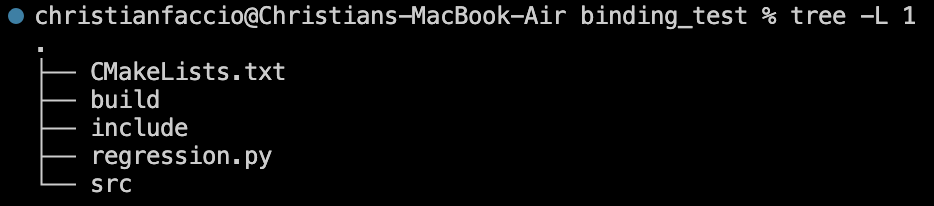
\includegraphics[width=0.8\textwidth]{assets/tree_bindings.png}
    \caption{Project organization}
    \label{fig:pybind11_project}
\end{figure}
here, the \texttt{src} folder contains the source files, the \texttt{include} folder contains the header files and the \texttt{build} folder is used for CMake.

We first start implementing the headers of the data-generation process (to create the dataset) and for the model fitting.

\begin{exampleblock}[Data-generation process]
    \begin{codeblock}[language=C++]
#ifndef DATAGEN_HPP
#define DATAGEN_HPP

#include <iostream>
#include <vector>
#include <set>
#include <random>
#include <map>

template <typename T>
std::map<T, T> generateData(const std::set<T> &x, const int n) {
    std::random_device rd;
    std::mt19937 gen(rd());
    std::normal_distribution<> d(0, 1);

    std::map<T, T> data;
    for (int i = 0; i < n; i++) {
        T x_val = *std::next(x.begin(), i % x.size());
        T y_val = x_val + d(gen);
        data[x_val] = y_val;
    }
    return data;
}

#endif // DATAGEN_HPP
    \end{codeblock}
\end{exampleblock}


\begin{exampleblock}[Model fitting]
    \begin{codeblock}[language=C++]
#ifndef REGRESSION_HPP
#define REGRESSION_HPP

#include <iostream>
#include <map>

class Regression {
public:
    Regression() = default;
    ~Regression() = default;

    template <typename T>
    void fit(const std::map<T, T> &data) {
        T x_mean = 0;
        T y_mean = 0;
        for (const auto &pair : data) {
            x_mean += pair.first;
            y_mean += pair.second;
        }
        x_mean /= data.size();
        y_mean /= data.size();

        T numerator = 0;
        T denominator = 0;
        for (const auto &pair : data) {
            numerator += (pair.first - x_mean) * (pair.second - y_mean);
            denominator += (pair.first - x_mean) * (pair.first - x_mean);
        }
        slope = numerator / denominator;
        intercept = y_mean - slope * x_mean;
    }

    template <typename T>
    T predict(const T &x) {
        return slope * x + intercept;
    }

    template <typename T>
    void print() {
        std::cout << "y = " << slope << "x + " << intercept << std::endl;
    }

private:
    double slope;
    double intercept;
};

#endif // REGRESSION_HPP
    \end{codeblock}
\end{exampleblock}

They have been implemented header-only and with templates to allow for different types of data.

\begin{observationblock}
    The following step should be to test if the written code performs as expected. We wrote the \plaintt{main.cpp} file to test the code.
    \begin{codeblock}[language=C++]
#include "../include/datagen.hpp"
#include "../include/regression.hpp"

#include <iostream>

int main() {
    // Generate data
    std::set<double> x = {1.5, 2.3, 3.1, 4.0, 5.5, 6.9, 7.1, 8.6, 9.2, 10.0};
    std::map<double, double> data = generateData(x, 100);

    // Fit the model
    Regression regression;
    regression.fit(data);

    // Print the model
    regression.print<int>();

    return 0;
        }
    \end{codeblock}
\end{observationblock}

The next step is to expose the C++ code to Python using pybind11. We start by creating a \texttt{bindings.cpp} file in the \texttt{src} folder.

\begin{exampleblock}[bindings.cpp]
\begin{codeblock}[language=C++]
#include <pybind11/pybind11.h>
#include <pybind11/stl.h>
#include "../include/datagen.hpp"   // Contains generateData function (without PYBIND11_MODULE)
#include "../include/regression.hpp" // Contains Regression class (without PYBIND11_MODULE)

namespace py = pybind11;

// Define a module that exposes both functionalities.
PYBIND11_MODULE(BindingTestModule, m) {
    m.doc() = "Combined data generation and regression module";

    // Bind datagen function.
    m.def("generateData", &generateData<int>, "Generate data for a given set of x values and n points");

    // Bind the Regression class.
    py::class_<Regression>(m, "Regression")
        .def(py::init<>())
        .def("fit", &Regression::fit<double>)
        .def("predict", &Regression::predict<double>)
        .def("print", &Regression::print<double>);
    }

\end{codeblock}
\end{exampleblock}

The module has been named \textbf{BindingTestModule} and contains the \texttt{generateData} function and the \texttt{Regression} class. The \texttt{fit}, \texttt{predict}, and \texttt{print} methods have been bound to the Python module.

It is time now to compile the code. We create a \texttt{CMakeLists.txt} file in the main directory.

\begin{exampleblock}[CMakeLists.txt]
\begin{codeblock}[language=C++]
cmake_minimum_required(VERSION 3.10)
project(BindingTest)

set(CMAKE_CXX_STANDARD 17)
set(PYBIND11_FINDPYTHON ON)
find_package(pybind11 REQUIRED)

include_directories(${CMAKE_CURRENT_SOURCE_DIR}/include)

# Create an executable for C++ tests if needed.
add_executable(BindingTestExe src/main.cpp)
target_include_directories(BindingTestExe PRIVATE include)

# Create one Python module target from bindings.cpp.
pybind11_add_module(BindingTestModule src/bindings.cpp)
target_link_libraries(BindingTestModule PRIVATE pybind11::pybind11)
\end{codeblock}
\end{exampleblock}

Now run the following commands in your terminal to compile the code:

\begin{codeblock}[language=bash]
mkdir build
cd build
cmake ..
make
\end{codeblock}

The compilation will create a shared library file named \texttt{BindingTestModule.cpython-312-darwin.so} in the \texttt{build} folder that can be imported into Python. 
The Python code to test the C++ code is as follows:

\begin{exampleblock}[regression.py]
\begin{codeblock}[language=python]
import sys 
sys.path.append('build')  # Add the build directory to the path
import BindingTestModule  # type: ignore # our combined module
import matplotlib.pyplot as plt
import numpy as np

# --- Generate sample data ---
# Create a set of x values. (Python sets will convert to C++ std::set.)
x_values = {1, 2, 3, 4, 5}
n_points = 50

# Call the data generation function from our module.
# This should return a dictionary mapping x values to y values.
data = BindingTestModule.generateData(x_values, n_points)

# Convert the dictionary to sorted lists for plotting.
x_data = sorted(data.keys())
y_data = [data[x] for x in x_data]

# --- Fit the regression model ---
# Create an instance of the Regression class from our module.
reg = BindingTestModule.Regression()
reg.fit(data)  # Fit using the generated data

# --- Prepare the regression line ---
# Create a smooth range of x values for plotting the regression line.
x_line = np.linspace(min(x_data) - 1, max(x_data) + 1, 100)
# Get predicted y values using the regression model.
y_line = [reg.predict(x) for x in x_line]

# --- Plotting the results ---
plt.figure(figsize=(8, 6))
plt.scatter(x_data, y_data, color='blue', label='Data Points')
plt.plot(x_line, y_line, color='red', label='Regression Line')
plt.xlabel('x')
plt.ylabel('y')
plt.title('Data and Regression Line')
plt.legend()
plt.grid(True)
plt.show()
\end{codeblock}
\end{exampleblock}

The Python code generates sample data, fits a regression model to the data, and plots the data points and the regression line. The data generation and regression fitting are performed using the C++ code exposed to Python.
The following image is generated:

\begin{figure}[H]
    \centering
    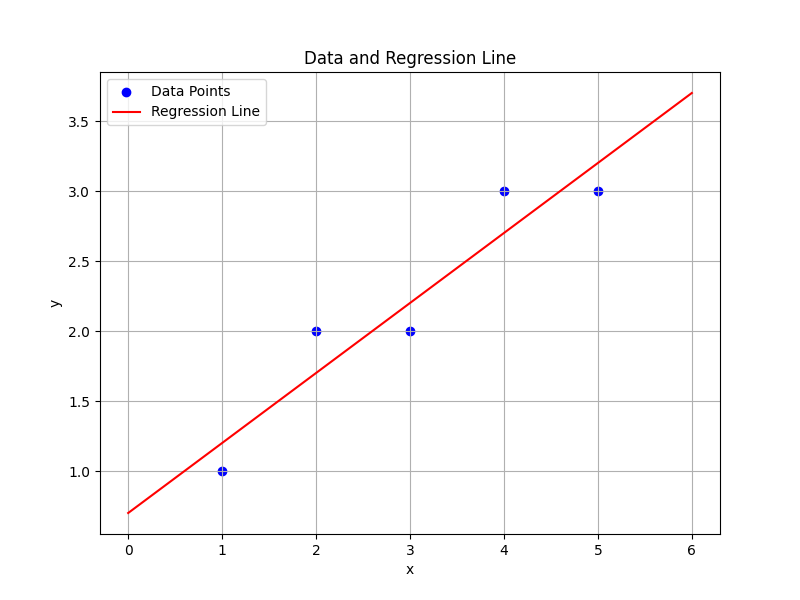
\includegraphics[width=0.8\textwidth]{assets/regression.png}
    \caption{Regression plot}
    \label{fig:regression}
\end{figure}




    